\chapter{Point de vue Utilisateur}

\section{Plugins developpés}
Middleware qui est notre plugin principal propose la vue Eclipse suivante : \textbf{image manquante}. 
\begin{description}
\item[Load Video]
L'utilisateur doit au préalable avoir renseigné le chemin de la vidéo à analyser. Le plugin Acquisition est sollicité au déclenchement de ce bouton. 
\item[Lancer Analyse]
Appel du plugin Reasoning qui effectue une analyse de la vidéo précedement acquise.
\item[Post]
L'utilisateur doit au préalable avoir renseigné l'acces token nécessaire pour poster sur une plateforme en ligne. 
Le plugin en charge de poster sur un blog ou un réseau social est appelé.
\end{description}
 
\section{Lancement du plugin et manuel d'utlisation}

Pour lancer le plugin suivez les étape suivante:

\begin{enumerate}
 \item Cliquer dans le menu sur \og Run \fg, puis et cliquer sur \og Run configuration \fg, 
afin d'offrir un fenêtre de configuration (cf\label{fig:fenetreConfg} ).
  \begin{figure}
	  \centering
	  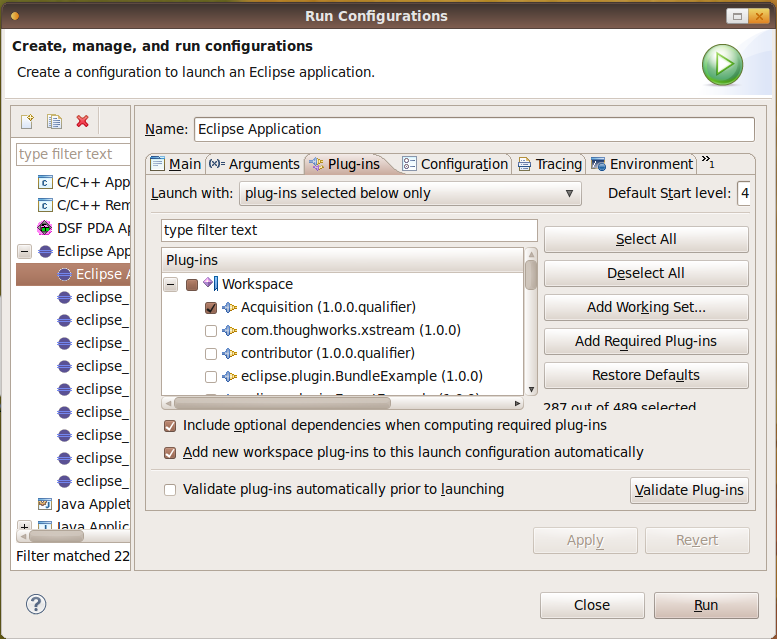
\includegraphics[scale=0.50]{img/tuto}
	  \caption{Fenêtre de configuration}
	  \label{fig:fenetreConfg}
\end{figure}

  \item Un fois la fenêtre ouverte cliquer sur l'onglet plugin et cocher les laber:
      \subitem Acquisition
      \subitem Middleware
      \subitem NetP
      \subitem Reasoning
\end{enumerate}


